\chapter{Setup}

Dieses Kapitel handelt von der Installation und Ersteinrichtung der Suchmaschine über Docker. Bei einem Meeting wurde beschlossen, dass ElasticSearch als Suchmaschine genutzt wird. Die Installation erfolgt dabei über Docker-Compose, zum Verwalten von mehreren Docker-Maschinen. Dabei werden 2 ElasticSearch Instanzen, eine Kibana Instanz und eine Logstash-Instanz verwendet. Um das System abzusichern wird zudem der Reverse-Proxy Traefik verwendet. Dabei wird Kibana mit SSL-Verschlüsselung und dem Login-System versehen. Auch die Anfragen an ElasticSearch werden mit einer Basic-Authenification gesichert.

\section{Docker}

Die Konfiguration der Instanzen funktioniert größtenteils über YAML-Datei. Dabei wird für jedes System die entsprechende Datei gemountet. 

Zudem möchte ich noch gern auf die Rechte-Verwaltung von Docker eingehen. Jeder Container kann seine eigenen Nutzer anlegen, jedoch können diese nicht unbedingt auf den Filesystem der Hosts schreiben. Um nun einen Docker-Container Nutzer das Recht zu geben auf den Filesystem zu schreiben, muss die User-ID der Datei auf denselben Wert gesetzt werden, wie der Nutzer im Container. ElasticSearch verwendet grundsätzlich einen Nutzer mit der UID 1000 und der GUID 1000. Deswegen müssen die Ordner auf dem Host-System nun auch diese Rechte bekommen. Dazu wurden mit CHOWN die Rechte auf 1000:1000 gesetzt. Allerdings ist der Nutzer 1000 auf dem Host-System ein anderer Nutzer. Deswegen besitzt jetzt ein anderer Nutzer die Dateien in den ElasticSerach Ordner. Um dies zu beheben, wurde der Nutzer auf eine andere UID/GUID gesetzt um Konfusion zu vermeiden. \cite{JarrodWeaver.2014}

\subsection{ElasticSearch}

\begin{lstlisting}[language=XML, frame=single, label={lst:es01}] 
	es01:
	image: docker.elastic.co/elasticsearch/elasticsearch:7.5.1
	container_name: es01
	environment:
		- "ES_JAVA_OPTS=-Xms4g -Xmx4g"
	ulimits:
		memlock: -1
	volumes:
		- /srv/elk/elasticSearch01/:/usr/share/elasticsearch/data
		- /srv/elk/config/elasticsearch.yml:
			/usr/share/elasticsearch/config/elasticsearch.yml
	ports:
		- 9200:9200
	networks:
		- elastic
\end{lstlisting}

Für die beiden ElasticSearch Instanzen wurde zudem der Java-Speicher erhöht. Es werden 4 Gigabyte benutzt, da wir 2 Server haben, welcher allerdings in Kombination niemals mehr Speicher verwenden sollen als 50 \% des gesamten RAMs. \cite{ElasticsearchB.V..12172019}

Der ulimits Befehl hebt die Begrenzung des Memory-Locks auf, damit ElasticSearch korrekt arbeiten kann.

Als Volumes ist zum einen die oben genannte YAML-Datei angegeben und zum anderen wird der Datenordner gemountet. Dies dient dazu, dass, falls der Container zerstört wird, die indexierten Daten trotzdem weiterhin gespeichert werden.

Der Port wird zum Host-System durchgereicht, damit das System auch von außerhalb des Docker-Netwerkes zu erreichen ist. Dabei ist das System troz blockierter UFW zu erreichen. Dies liegt daran, dass Docker in der Standardeinstellung UFW ignoriert.

In der ElasticSearch-Konfigurationsdatei werden nun die Einstellungen, die speziell für das ElasticSearch-System relevant sind verwaltet. 

Darin wird zuerst der Cluster-Name definiert. Dieser dient dazu, dass die Server wissen, dass Sie dieselben Daten betreuen. 
Danach wird der Name des Servers vergeben. Dieser wird für spätere Einstellungen noch wichtig.

Das Memory-Lock Setting dient dazu, dass die Anwendung verhindert, dass sie in den SWAP gelegt wird. Laut ElasticSearch-Website bricht die Suchgeschwindigkeit ein, sollte das Programm in den SWAP gelegt werden.

Der Network Host wird hier auf alle Interfaces der Maschine gesetzt, damit sich alle System innerhalb der Docker Netzwerkes finden können.
Das Seed-Host Setting sagt aus, an welche Nodes die Daten synchronisiert werden sollen.

Der letzte Eintrag dient dazu, dass bei der ersten Synchronisation das System weiß, welche Nodes alle Daten enthalten, also mit welchen Server sich synchronisiert werden soll. Da hier beide Systeme beim ersten Start noch keine Daten besitzen, sind alle Nodes zu beginnt Master. 
\begin{lstlisting}[language=XML, frame=single, label={lst:es01-yml}] 
	cluster.name: dietrich-online-cluster
	node.name: es01
	bootstrap.memory_lock: true
	network.host: 0.0.0.0
	discovery.seed_hosts: ["es02"]
	cluster.initial_master_nodes: ["es01", "es02"]
\end{lstlisting}

\subsection{Kibana}

Die Grundkonfiguration von Kibana ist einfacherer als die Konfiguration von ElasticSearch. Es muss nur die YAML-Datei gemountet werden und der Port 5601 nach außen durchgereicht werden.

In der YAML-Datei werden nun die Einstellungen für Kibana gesetzt. Darunter fällt der oben genannte Port, der Server-Host, in diesem Fall auch 0.0.0.0, damit Kibana auf alle Interfaces innerhalb des Containers hört, und die ElasticSearch-Hosts. Dabei werden alle Server Instanzen mitgegeben, auf denen Kibana arbeiten soll. 

\subsection{Logstash}

Für die Grundkonfiguration von Logstash muss, wie schon im Test vorher, der Treiber in die Core-Bibliothek gemountet werden. Zudem wird ein Ordner gemountet, in dem alle Conf-Dateien für die Pipeline geladen werden. Dieser Ordner wird dann alphabetisch von Logstash abgearbeitet. In der YAML wird dann der Name, die Pipeline.id und die Pipeline-Worker festgelegt. Die Pipeline-Worker sind die Threads in denen eine der eben genannten Conf-Dateien bearbeitet wird. Generell sollte die Anzahl der Cores auch die maximale Anzahl der Worker sein.


\section{X-Security}

X-Security nennt sich das Paket mit den Sicherheitseinstellungen vom ELK-Stack. Dafür habe ich hier den kompletten Traffic zwischen den einzelnen Komponenten, sowie der Endnuzter zum Server mit SSL verschlüsselt. Dazu mussten zuerst einmal die Zertifikate generiert werden. Dafür bietet ElasticSearch ein Tool an, welches eine Autorität und die einzelnen Zertifikate mit Private und Public-Key generiert. Allerdings werden diese standardmäßig im PKCS 12-Format (FOOTNOTE) abgespeichert. Dieses ist ein Container-Format, welches die Schlüssel und die Autorität zusammen verpackt. Jedoch benötigt Kibana zum Beispiel nur die Autorität als einzelnes Zertifikat und nicht in einem Container.

Es gibt eine Möglichkeit diese Dateien aus der PK12 zu entpacken, jedoch gab es auch hierbei Probleme, da OpenSSL, das Tool welches zum Entpacken verwendet wird, die Autorität nicht richtig entpackt. \cite{nerophon.2018}

Es kann allerdings auch bei der Zertifikat-Erstellung eine Option mitgegeben werden, dass die Zertifikate nicht verpackt werden sollen. Um nun alle Zertifikate gleichzeitig zu generieren, kann eine YAML Datei mitgegeben werden, welche alle Informationen zu den einzelnen Systemen enthält. In diesem Fall wurde nur der DNS-Name angegeben \ref{lst:certs-yml}. Mit diesen Informationen wurde nun für alle Systeme Zertifikate generiert. 

\begin{lstlisting}[language=XML, frame=single, label={lst:certs-yml}] 
	instances:
	- name: 'es01'
	  dns: [ 'es01', 'bib55', 'bib55.uni-trier.de' ]
	  [...]
\end{lstlisting}

Um die Zertifikate nun einzutragen, mussten nur in den diversen YAML-Dateien alle Pfade angegeben werden. 

Zusätzlich zu den Zertifikaten muss auch noch eine Password Authentifikation eingebaut werden. Dazu kann auf den ElasticSearch-Containern ein Befehl zur Erstellung der Systempasswörter aufgerufen werden. Diese müssen dann auch in den YAML-Dateien vermerkt werden. Weitere Nutzer können dann per API oder Kibana erstellt werden. Die Verteilung der Rechte passiert hierbei rollen-basiert. Es wird zuerst eine Rolle erstellt, mit den gewünschten Rechten, welche daraufhin an den Nutzer weitergegeben wird.

Um nun einen Query gegen das ElasticSearch System zu stellen, muss zum einen eine BasicAuth sowie das Zertifikat mitgegeben werden \ref{lst:curlQuery}.

\begin{lstlisting}[language=BASH, frame=single, label={lst:curlQuery}] 
	curl https://bib55:9200 --cacert ca.crt -uuser:pass
\end{lstlisting}

Um nun die Daten mit Logstash einzuspielen, wurde ein Nutzer erstellt, welcher nur Zugriff auf Indices mit dem Präfix dietrich\_ und die Logstash-Indices besitzt. Diese Einstellungen konnten alle über die Benuzter-Oberfläche von Kibana gemacht werden \ref{img:kibanaRoles}. 


\begin{figure}
	\centering
	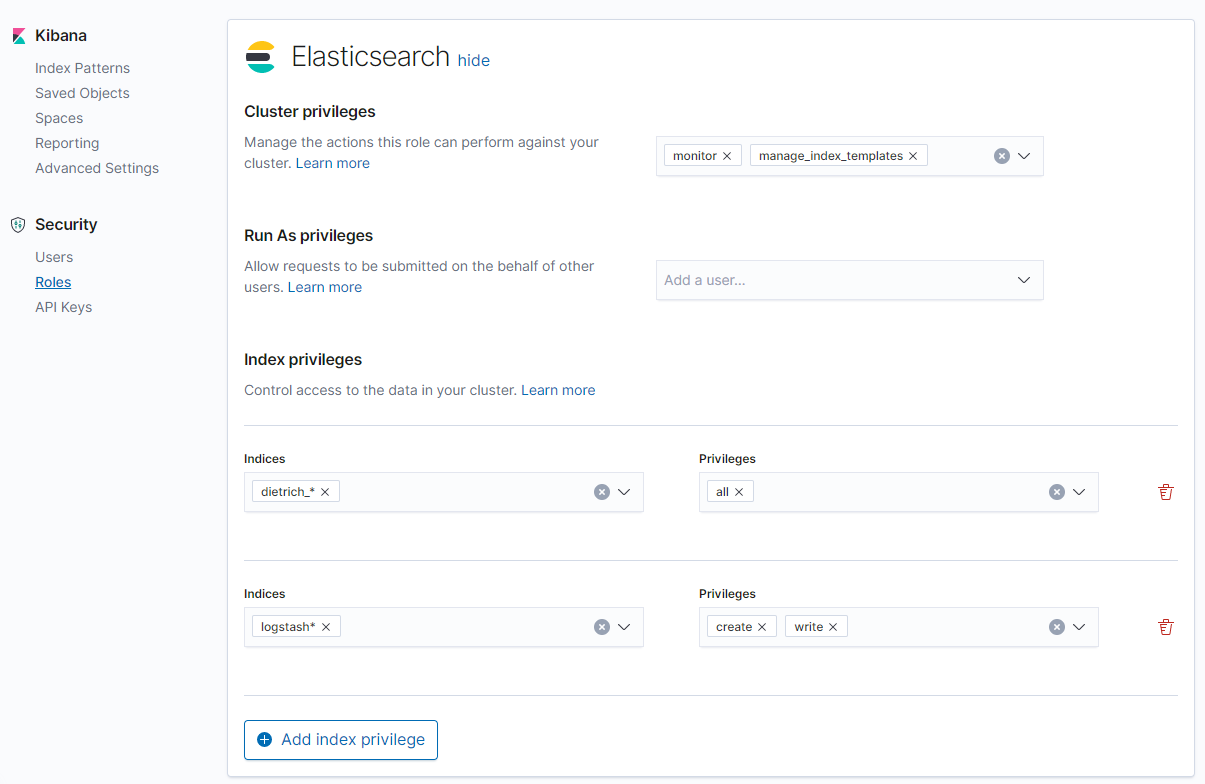
\includegraphics[width=1\linewidth]{images/setup/kibana_roles.png}
	\caption{Seite zu Erstellung von Rechte-Rollen}
	\label{img:kibanaRoles}
\end{figure}

\subsection{Vollständiges Setup}

GRAFIK